\documentclass[11pt,a4paper]{article}

% Packages for encoding and typography
\usepackage[utf8]{inputenc}
\usepackage{fontenc}
\usepackage{lmodern}
\usepackage[margin=1in]{geometry}
\usepackage{graphicx}
\usepackage{booktabs}
\usepackage{amsmath}
\usepackage{titlesec}
\usepackage{xcolor}
\usepackage{hyperref}

% TikZ for diagrams
\usepackage{tikz}
\usetikzlibrary{shapes.geometric, arrows.meta, positioning}

% Customizing section titles for a professional look
\titleformat{\section}{\Large\bfseries\color{blue!70!black}}{\thesection}{1em}{}
\titleformat{\subsection}{\large\bfseries\color{blue!60!black}}{\thesubsection}{1em}{}

% Hyperlink configuration
\hypersetup{
    colorlinks=true,
    linkcolor=blue!70!black,
    urlcolor=blue!70!black,
}

\title{\textbf{BMEN4460\\
    Project Proposal: Patient-Customized Counterfactual Data Augmentation via Latent Drifting}}
\author{Thomas Moulin (tmm2219)}
\date{}


\begin{document}

\maketitle

\section{Global Vision and Concrete Proof of Concept}

\subsection{The Universal ''Slider'' Framework (Global Vision)}
The ambition of this project is to develop a universal, multi-conditional generative framework. By utilizing Latent Drifting within a Cycle Diffusion model, we aim to create a system equipped with clinical ''sliders''. This architecture allows researchers to continuously adjust a conditioning vector containing variables such as Age, or the presence of Alzheimer's Disease ($A_D$), Amyotrophic Lateral Sclerosis (ALS), and Frontotemporal Dementia (FTD). By manipulating these parameters, the model can simulate personalized structural brain changes, showing how a specific patient's brain would evolve under various neurodegenerative conditions. This counterfactual tool is especially vital for rare diseases like ALS and FTD, where longitudinal imaging data is severely lacking.

\subsection{Concrete Proof of Concept (Project Scope)}
While the theoretical architecture is designed to be globally scalable across multiple pathologies, the concrete implementation and validation for this two-month project will serve as a targeted proof of concept focusing exclusively on Alzheimer's Disease ($A_D$) versus Cognitively Normal ($C_N$) states.
\begin{itemize}
    \item \textbf{Datasets:} The practical implementation utilizes the OASIS-1, OASIS-2, and OASIS-3 datasets, which serve as standard benchmarks for healthy aging and dementia.
    \item \textbf{Modalities and View:} The project extracts 2D Axial slices from 3D T1-weighted (T1W) and resting-state fMRI (rs-fMRI) volumes to ensure rapid iterations within the timeframe.
\end{itemize}

\begin{figure}[ht]
    \centering
    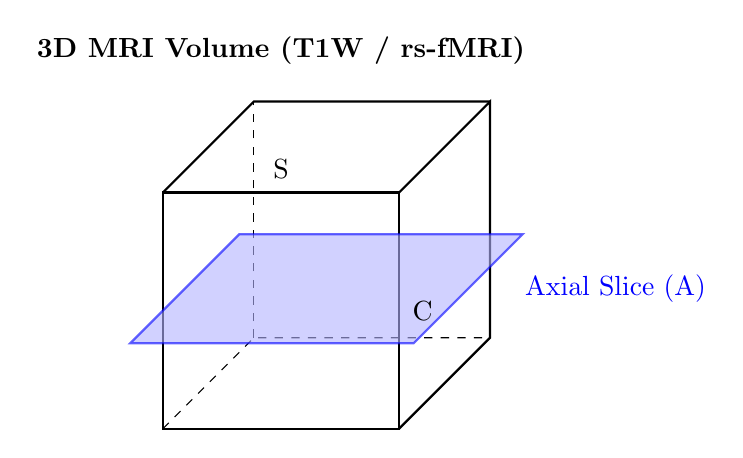
\begin{tikzpicture}[scale=1.5]
    % 3D Cube
    \draw[thick] (0,0,0) -- (2,0,0) -- (2,2,0) -- (0,2,0) -- cycle;
    \draw[thick] (2,0,0) -- (2,0,-2) -- (2,2,-2) -- (2,2,0);
    \draw[thick] (0,2,0) -- (0,2,-2) -- (2,2,-2);
    \draw[dashed] (0,0,0) -- (0,0,-2) -- (2,0,-2);
    \draw[dashed] (0,0,-2) -- (0,2,-2);

    % Axial Plane
    \filldraw[fill=blue!30, draw=blue, thick, opacity=0.6] (-0.2,0.8,0.2) -- (2.2,0.8,0.2) -- (2.2,0.8,-2.2) -- (-0.2,0.8,-2.2) -- cycle;

    % Labels
    \node[blue, right] at (2.6,0.8,-1) {Axial Slice (A)};
    \node at (2.2, 1, 0) {C}; % Coronal
    \node at (1, 2.2, 0) {S}; % Sagittal
    \node[above] at (1,3,0) {\textbf{3D MRI Volume (T1W / rs-fMRI)}};
    \end{tikzpicture}
    \caption{Extraction of 2D Axial slices from 3D MRI volumes for the downstream 2D pipeline.}
\end{figure}

\section{Technical Methodology: The 3-Step Pipeline}
The project relies on a three-step comparative methodology to validate the generative approach on the $A_D$ proof of concept:

\subsection{Step 1: 2D $A_D$ Classifier Baseline}
A standard 2D classifier will first be trained to distinguish between real $A_D$ and real $C_N$ images. This network serves as the ultimate benchmark to evaluate the clinical validity of the synthetic counterfactual images.

\begin{figure}[ht]
    \centering
    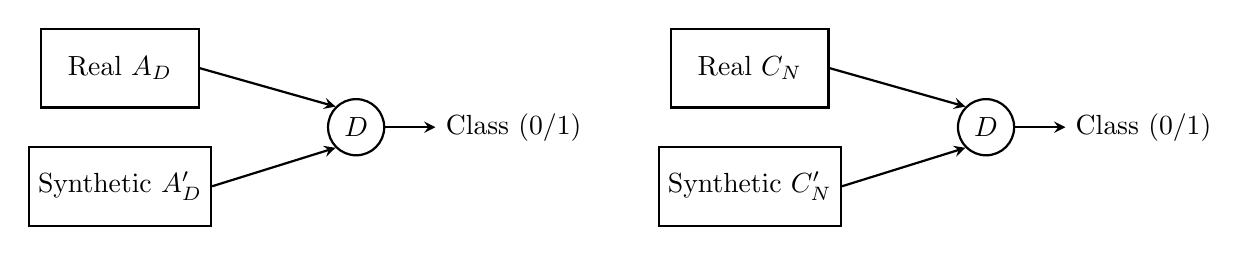
\begin{tikzpicture}[node distance=2.5cm, thick]
    % Left side: AD classifier validation
    \node[draw, rectangle, minimum width=2cm, minimum height=1cm] (RealAD) at (0,0) {Real $A_D$};
    \node[draw, rectangle, minimum width=2cm, minimum height=1cm] (FakeAD) at (0,-1.5) {Synthetic $A_D'$};
    \node[draw, circle] (D) at (3,-0.75) {$D$};
    \node (Pred) at (5,-0.75) {Class (0/1)};

    \draw[->, >=stealth] (RealAD.east) -- (D.north west);
    \draw[->, >=stealth] (FakeAD.east) -- (D.south west);
    \draw[->, >=stealth] (D.east) -- (Pred.west);

    % Right side: CN classifier validation
    \node[draw, rectangle, minimum width=2cm, minimum height=1cm] (RealCN) at (8,0) {Real $C_N$};
    \node[draw, rectangle, minimum width=2cm, minimum height=1cm] (FakeCN) at (8,-1.5) {Synthetic $C_N'$};
    \node[draw, circle] (D2) at (11,-0.75) {$D$};
    \node (Pred2) at (13,-0.75) {Class (0/1)};

    \draw[->, >=stealth] (RealCN.east) -- (D2.north west);
    \draw[->, >=stealth] (FakeCN.east) -- (D2.south west);
    \draw[->, >=stealth] (D2.east) -- (Pred2.west);
    \end{tikzpicture}
    \caption{Validation strategy using a 2D Classifier ($D$) evaluating both real and synthetically drifted images.}
\end{figure}

\subsection{Step 2: CycleGAN + Swin UNET}
Before utilizing diffusion, a CycleGAN integrated with a Swin UNET architecture will be implemented. This serves as a baseline for unpaired image-to-image translation.

\subsection{Step 3: Cycle Diffusion with Latent Drifting (Core Innovation)}
Instead of translating images directly in the pixel space, a patient's MRI is encoded into a compressed latent space. Using Latent Drifting, the condition vector (acting as the ''sliders'') is manipulated to simulate how that specific patient's brain would evolve under the targeted clinical condition.

\pagebreak
\section{The Counterfactual Framework Mechanism}
The counterfactual generation mechanism operates via dual cycles ($A_D \rightarrow C_N' \rightarrow A_D''$ and $C_N \rightarrow A_D' \rightarrow C_N''$) ensuring strict morphological preservation of the patient's identity.

\begin{figure}[ht]
    \centering
    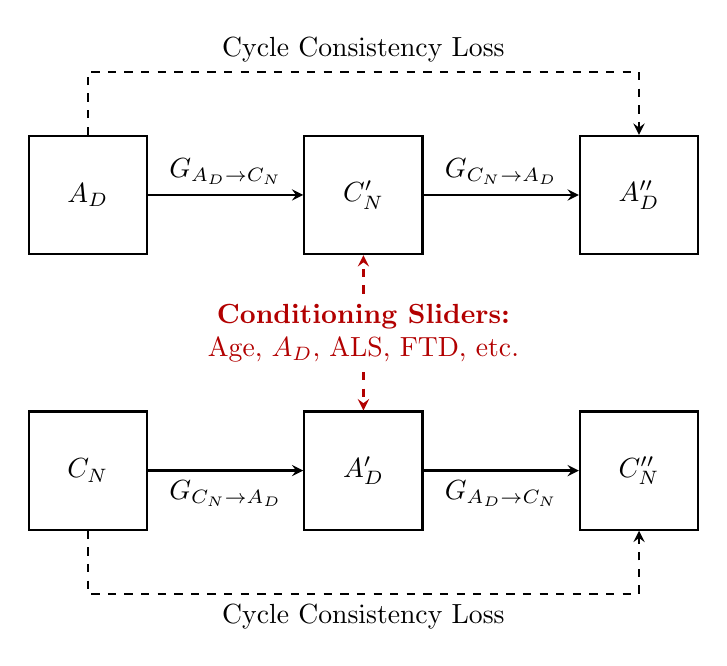
\begin{tikzpicture}[thick]
    % Nodes for Cycle 1 (AD to CN)
    \node[draw, rectangle, minimum width=1.5cm, minimum height=1.5cm] (AD) at (0, 0) {$A_D$};
    \node[draw, rectangle, minimum width=1.5cm, minimum height=1.5cm] (CNp) at (3.5, 0) {$C_N'$};
    \node[draw, rectangle, minimum width=1.5cm, minimum height=1.5cm] (ADpp) at (7, 0) {$A_D''$};

    % Arrows for Cycle 1
    \draw[->, >=stealth] (AD) -- node[above] {$G_{A_D \rightarrow C_N}$} (CNp);
    \draw[->, >=stealth] (CNp) -- node[above] {$G_{C_N \rightarrow A_D}$} (ADpp);
    \draw[->, dashed, >=stealth] (AD.north) -- +(0,0.8) -| node[above, pos=0.25] {Cycle Consistency Loss} (ADpp.north);

    % Nodes for Cycle 2 (CN to AD)
    \node[draw, rectangle, minimum width=1.5cm, minimum height=1.5cm] (CN) at (0, -3.5) {$C_N$};
    \node[draw, rectangle, minimum width=1.5cm, minimum height=1.5cm] (ADp) at (3.5, -3.5) {$A_D'$};
    \node[draw, rectangle, minimum width=1.5cm, minimum height=1.5cm] (CNpp) at (7, -3.5) {$C_N''$};

    % Arrows for Cycle 2
    \draw[->, >=stealth] (CN) -- node[below] {$G_{C_N \rightarrow A_D}$} (ADp);
    \draw[->, >=stealth] (ADp) -- node[below] {$G_{A_D \rightarrow C_N}$} (CNpp);
    \draw[->, dashed, >=stealth] (CN.south) -- +(0,-0.8) -| node[below, pos=0.25] {Cycle Consistency Loss} (CNpp.south);

    % Conditioning variables (The Sliders)
    \node[text=red!70!black, align=center] (cond) at (3.5, -1.75) {\textbf{Conditioning Sliders:}\\Age, $A_D$, ALS, FTD, etc.};
    \draw[->, red!70!black, dashed, >=stealth] (cond) -- (CNp.south);
    \draw[->, red!70!black, dashed, >=stealth] (cond) -- (ADp.north);

    \end{tikzpicture}
    \caption{Cycle Diffusion Framework. The latent vector acts as multiple "sliders" allowing the synthesis of various counterfactual states while preserving the core patient identity.}
\end{figure}


\section{Scientific Impact}
This approach steps away from traditional, random data augmentation. By bridging Latent Drifting with Cycle Diffusion, the project tackles the distribution shift problem directly in the latent space. Generating high-fidelity counterfactuals allows for synthetically expanding the dataset with personalized disease progression maps, proving the feasibility of a universal tool that could eventually map multiple neurodegenerative diseases.

\end{document}